\section{Considerations on Grain Boundaries}\label{sec:grain-boundaries}

In contrast to free surfaces, where the geometric evolution of a node is not constrained by the surrounding space, in grain boundaries the node shifting acts counter the solid material of the other particle.
This introduces additional constraints, since the grain boundary must not form holes and must not overlap.
The geometric constraints are dependent on the local evolution of the grain boundary nodes, as well as the relative position change of the particles.

Starting from a compact grain boundary, meaning that there are no holes and/or overlap present within it, the condition of maintaining the compactness of the grain boundary can be formulated as follows, if the postions of the particles are fixed.

\begin{align}
    \Left{\Normal\ShiftStep} &= &-\Right{\Normal\ShiftStep} \\
    \Left{\Tangential\ShiftStep} &= &-\Right{\Tangential\ShiftStep}
    \label{eq:maintain-compact-particles-fixed}
\end{align}

But in reality the positions of particles to each other change, which can be observed macroscopically as shrinkage.
However, the relation between node shifting and particle movement cannot be easily formulated, since the particle movement is effected by the ensemble of all nodes involved in the contact.
But, we can formulate the influence of shifting one node in normal or tangential direction on the opposite particle, if that particle is assumed as invariant in shape.
Each contact node has two sets of coordinates, one in the terms of the one particle, one in terms of the other.
However, they represent both the same point in space.


\begin{figure}
    \centering
    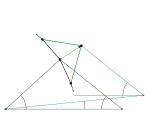
\includegraphics{img/model_development/particle_shift_normal}
    \caption{Effect of Normal Node Shifting on Particle Postion}
    \label{fig:model_development/particle_shift_normal}
\end{figure}

\begin{figure}
    \centering
    \includegraphics{img/model_development/particle_shift_tangential}
    \caption{Effect of Tangential Node Shifting on Particle Postion}
    \label{fig:model_development/particle_shift_tangential}
\end{figure}

\autoref{fig:model_development/particle_shift_normal} and \autoref{fig:model_development/particle_shift_tangential} show the geometric conditions of such a shift.
The left particle (index $\Left{\square}$) changes its shape by shifting a single regarded node, while the right particle (index $\Right{\square}$) is invariant.
The particles are assumed to be solely connected in the regarded node, the influence of adjacent nodes is disregarded.
Therefore, the radius line of the node regarded from the right particle retains the same length and angle to the surface normal of the node.
This is equivalent to a parallel shifting of the radius line to the tip of the shift vector $\vect\ShiftStep$.
It is obvious from the drawing, that under these conditions, the particles center must perform the same shift as the node, so $\vect\ShiftStep$ also describes the movement of the particles center.

The total movement of the right particle due to node shifting can be formulated as follows:
\begin{subequations}
    \begin{align}
        \Particle\RadiusStep &= \frac{\partial \Particle\Radius}{\partial \Normal\Shift} \Normal\ShiftStep + \frac{\partial \Particle\Radius}{\partial \Tangential\Shift} \Tangential\ShiftStep \\
        \Particle\AngleStep &= \frac{\partial \Particle\Angle}{\partial \Normal\Shift} \Normal\ShiftStep + \frac{\partial \Particle\Angle}{\partial \Tangential\Shift} \Tangential\ShiftStep \\
        \Particle\RotationAngleStep &= \frac{\partial \Particle\RotationAngle}{\partial \Normal\Shift} \Normal\ShiftStep + \frac{\partial \Particle\RotationAngle}{\partial \Tangential\Shift} \Tangential\ShiftStep
    \end{align} \label{eq:particle-steps}
\end{subequations}
The partial derivatives therein are obtained from the geometric relations in the above figures.

\begin{equation}
    \frac{\partial \Particle{\Radius}}{\partial \Normal\Shift}
    = \lim_{\Normal{\ShiftStep} \rightarrow 0}
    \frac{\Particle\Radius'-\Particle\Radius}{\Normal\ShiftStep}
    \label{eq:partial-particle-radius-node-normal}
\end{equation}

\begin{equation}
    \frac{\partial \Particle{\Angle}}{\partial \Normal\Shift}
    = \lim_{\Normal{\ShiftStep} \rightarrow 0}
    \frac{\Particle\AngleStep}{\Normal\ShiftStep}
    \label{eq:partial-particle-angle-node-normal}
\end{equation}

\begin{equation}
    \frac{\partial \Particle{\Radius}}{\partial \Tangential\Shift}
    = \lim_{\Tangential{\ShiftStep} \rightarrow 0}
    \frac{\Particle\Radius'-\Particle\Radius}{\Tangential\ShiftStep}
    \label{eq:partial-particle-radius-node-tangential}
\end{equation}

\begin{equation}
    \frac{\partial \Particle{\Angle}}{\partial \Tangential\Shift}
    = \lim_{\Tangential{\ShiftStep} \rightarrow 0}
    \frac{\Particle\AngleStep}{\Tangential\ShiftStep}
    \label{eq:partial-particle-angle-node-tangential}
\end{equation}

Of course, for each node the resulting movement of the particle will be different due to geometric relations and diffusive fluxes.
The geometric relations are fixed for a regarded state, but the diffusive fluxes can be used to fulfill \autoref{eq:particle-steps} simultaneously for all nodes involved in a contact.
So there is a set of equations available to describe particle contact conditions as constraints for the TEP-approach.